\documentclass[11pt, a4paper,twocolumn]{jarticle}
\usepackage[dvipdfmx]{graphicx}
\begin{document}
%=============================================================
\section{Inverting and non-inverting amplifiers ($3^{rd} day$)}
\subsubsection{Purpose}
実際の増幅器の基礎的な動作を理解するために,反転増幅回路,非反転増幅回路を製作し,それらの直流電流特性を調べる.
\subsection{Equipment}
\begin{itemize}
    \item 実験2と同様のもの
\end{itemize}
\subsubsection{Procedure}
まず反転増幅回路を図\ref{fig:10}のように作る.
今回の実験ではまず抵抗の値を$R_1=100k\Omega,R_2=10K\Omega$とする.
またDC-DCコンバーターを用いてオペアンプの電源としてパワーライン(+15V,-15V)を作る.
この際パワーラインとGNDの間に0.1$\mu$Fのコンデンサを挟むことを確認する.
回路を作った後入出力特性を電圧計を用いて計測する.
その後抵抗の値を$R_1=200k\Omega,R_2=10K\Omega$として再び入出力電圧を測定しどのように動作が変わるのかを観察する.

次に図\ref{fig:11}に示すように反転増幅回路を作る.
まずは抵抗の値を$R_1=100k\Omega,R_2=10K\Omega$とする.
その後先ほどの実験と同様に入出力電圧を測定した.
次に$R_1=200k\Omega,R_2=10K\Omega$として再び入出力電圧を測定する.

計測が終了した後それぞれの抵抗値の場合について入力電圧,出力電圧の関係をグラフにプロットして動作の違いや増幅率について調べる.

\begin{figure}[htbp]
 \begin{center}
  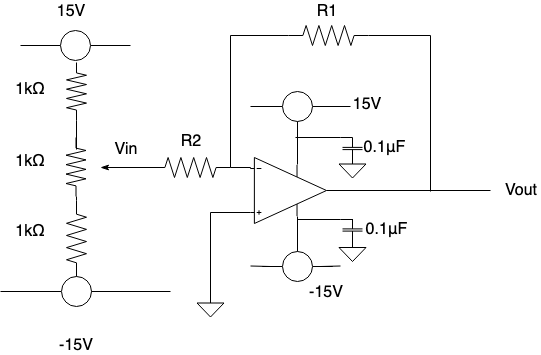
\includegraphics[width=0.8\linewidth]{fig10.png}
 \end{center}
 \caption{反転増幅回路}
 \label{fig:10}
\end{figure}


\begin{figure}[htbp]
 \begin{center}
  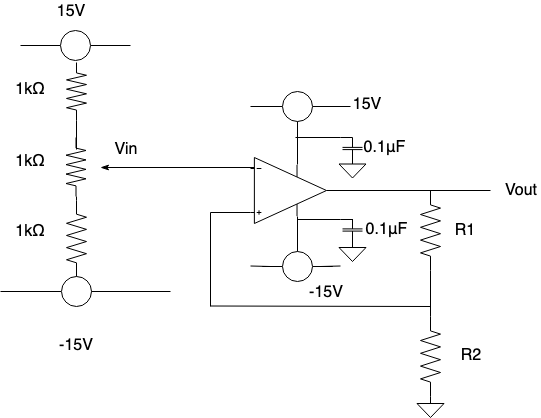
\includegraphics[width=0.8\linewidth]{fig11.png}
 \end{center}
 \caption{非反転増幅回路}
 \label{fig:11}
\end{figure}
\newpage

\subsubsection{Result}
測定結果よりグラフに描画したところ図\ref{fig:19},図\ref{fig:20},図\ref{fig:21},図\ref{fig:22}のようなグラフが得られた.
また増幅後の出力電圧が13.5Vを超え始めたあたりから増幅されずそれ以降は出力電圧が一定値をとるようになった.

さらにこれらの一定値を除いた測定値を用いてそれぞれのグラフにおいて最小二乗法を用いて傾きを求め,増幅率を求めた結果を以下に示す.

図\ref{fig:19} $R_1=100k\Omega,R_2=10k\Omega$の時 

$V_{out}/V_{in}=-10.046$

図\ref{fig:20} $R_1=200k\Omega,R_2=10k\Omega$の時 

$V_{out}/V_{in}=-20.248$

図\ref{fig:21} $R_1=100k\Omega,R_2=10k\Omega$の時 

$V_{out}/V_{in}=11.035$

図\ref{fig:19} $R_1=50k\Omega,R_2=10k\Omega$の時 

$V_{out}/V_{in}=6.0141$

\newpage

\begin{figure}[htbp]
 \begin{center}
  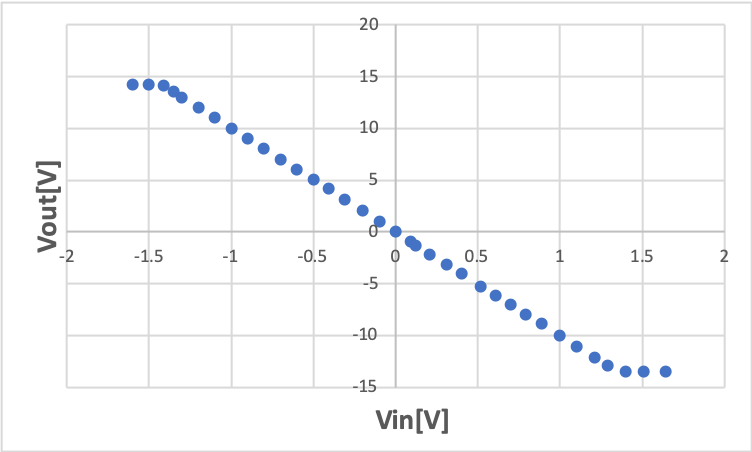
\includegraphics[width=0.8\linewidth]{fig19.png}
 \end{center}
 \caption{反転増幅回路($R_1=100k\Omega,R_2=10k\Omega$)}
 \label{fig:19}
\end{figure}

\begin{figure}[htbp]
 \begin{center}
  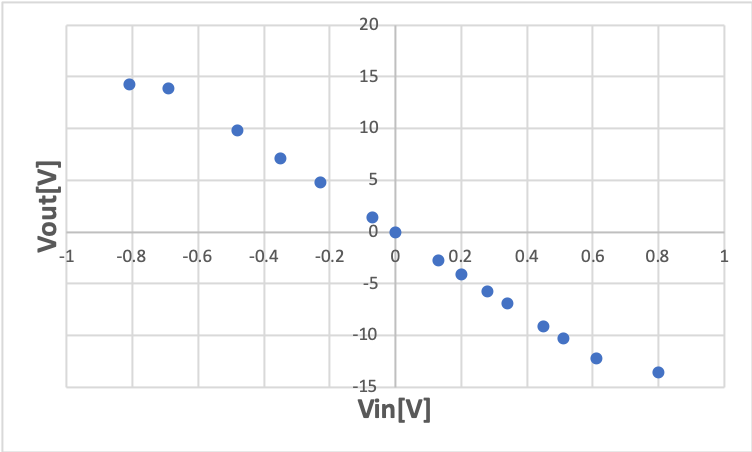
\includegraphics[width=0.8\linewidth]{fig20.png}
 \end{center}
 \caption{反転増幅回路($R_1=200k\Omega,R_2=10k\Omega$)}
 \label{fig:20}
\end{figure}

\newpage

\begin{figure}[htbp]
 \begin{center}
  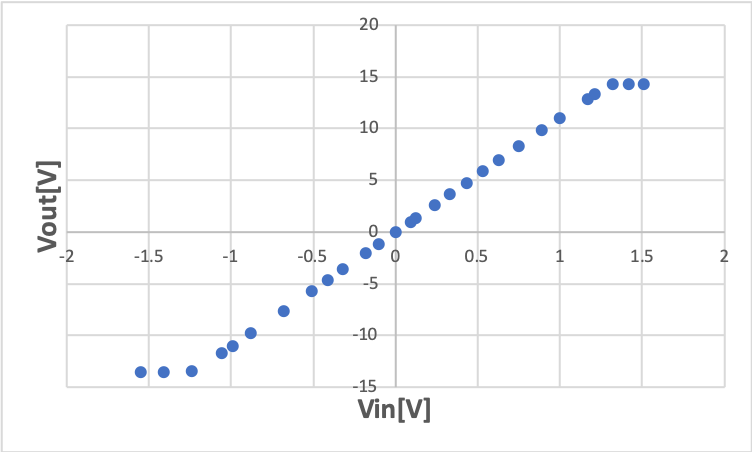
\includegraphics[width=0.8\linewidth]{fig21.png}
 \end{center}
 \caption{非反転増幅回路($R_1=100k\Omega,R_2=10k\Omega$)}
 \label{fig:21}
\end{figure}

\begin{figure}[htbp]
 \begin{center}
  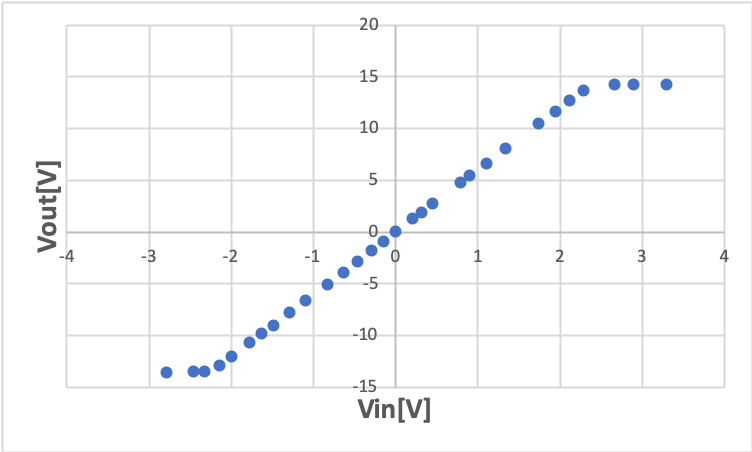
\includegraphics[width=0.8\linewidth]{fig22.png}
 \end{center}
 \caption{非反転増幅回路($R_1=50k\Omega,R_2=10k\Omega$)}
 \label{fig:22}
\end{figure}

\subsubsection{Discussion}
まず出力電圧が13V付近を境に一定値となってしまった原因としては今回使用したオペアンプは$\pm$15Vを電源として作動しているのでその電源電圧以上に増幅させることができないためだと考えられる.

また,なぜ非反転増幅回路,反転増幅回路がオペアンプにより実現できるのかについて考察する.
まず理想オペアンプとは
\begin{itemize}
    \item (性質1) 入力端子のインピーダンスが無限大であり,入力端子には電流が流れない.
    \item (性質2) 出力インピーダンスが0であり,出力電圧は出力電流に依存しない.
    \item (性質3) 電圧増幅率が無限大であり,オペアンプの入力電圧を$V_+,V_-$とすると$V_{out}$が有限値をとる時$V_+=V_-$の関係が成り立つ.
\end{itemize}
以上3つの特性をもつ.
この事実と図\ref{fig:10},図\ref{fig:11}の回路においてキルヒホッフの法則を使うと,

反転増幅回路の増幅率は次のように与えられ
\begin{equation}
    V_{out} = -\frac{R_1}{R_2}V_{in}
\end{equation}

非反転増幅回路の増幅率は次のように与えらる
\begin{equation}
    V_{out} = \left(1+\frac{R_1}{R_2}\right)V_{in}
\end{equation}
この式に図\ref{fig:19},図\ref{fig:20},図\ref{fig:21},図\ref{fig:22}の場合における抵抗の値を代入して増幅率を求めると,

図\ref{fig:19} $R_1=100k\Omega,R_2=10k\Omega$の時 

$V_{out}/V_{in}=-10$

図\ref{fig:20} $R_1=200k\Omega,R_2=10k\Omega$の時 

$V_{out}/V_{in}=-20$

図\ref{fig:21} $R_1=100k\Omega,R_2=10k\Omega$の時 

$V_{out}/V_{in}=11$

図\ref{fig:19} $R_1=50k\Omega,R_2=10k\Omega$の時 

$V_{out}/V_{in}=6$

となり概ね実験値と一致することが確かめられた.
図\ref{fig:20} $R_1=200k\Omega,R_2=10k\Omega$の値が実験値と理論値で一番大きな開きが生じてしまった理由としては,$200k\Omega$の抵抗がなかったために$100k\Omega$の抵抗2個を直列につなぎ代用したために抵抗値に若干のズレが生じてしまったことなどが考えられる.

またこれらの増幅器の応用例としては,入力として与えられた微弱な入力信号を増幅して取り出すことなどが挙げられる.
%=============================================================
\newpage
\end{document}
